\documentclass{article}
\usepackage[shortlabels]{enumitem}
\usepackage{pgfplots}
\usepgfplotslibrary{fillbetween}

\newcommand{\mathcolorbox}[2]{\colorbox{#1}{$\displaystyle #2$}}

\newtheorem{definition}{Definition}

\begin{document}	


\begin{definition}
Fläche zwischen zwei Graphen:
\[A = |\int_a^b f(x) dx - \int_a^b g(x) dx| = |\int_a^b f(x) - g(x) dx|\]

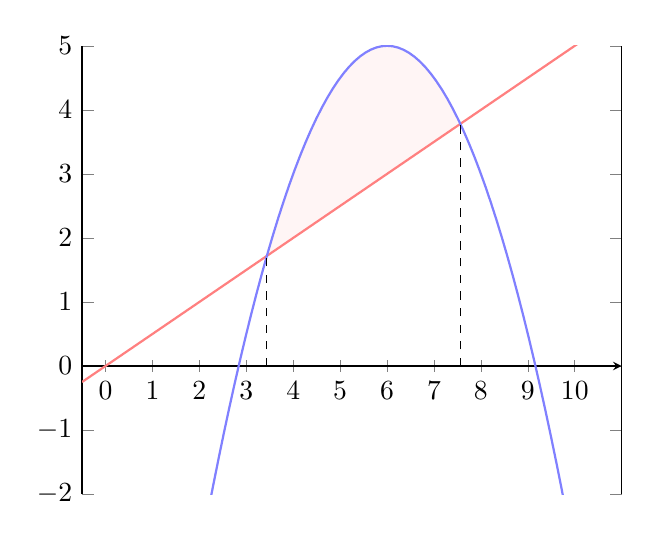
\begin{tikzpicture} 
   \begin{axis}[
      domain=-0.5:11,  
      xmin=-0.5, xmax=11, xtick={0,1, ..., 11},
      ymin=-2, ymax=5, ytick={-2, -1, ..., 5},
        axis x line=center, 
      ] 
      
     \addplot [samples=500, name path=f, thick, color=red!50]
        {0.5*x};

    \addplot [samples=100, name path=g, thick, color=blue!50]
        {- 0.5*(x-6)^2+5};

    \addplot[red!10, opacity=0.4] fill between[of=f and g, soft clip={domain=3.5:7.5}];

    \draw [dashed] (axis cs:{3.44,0}) -- (axis cs:{3.44,1.72});
    \draw [dashed] (axis cs:{7.56,0}) -- (axis cs:{7.56,3.78});
      
   \end{axis} 
\end{tikzpicture} 

\end{definition}

\begin{definition}

Seien f, g stletige Funktionen auf I = [a;b] und $ f(x) \geq g(x) $ für alle $ x \in I = [a;b]$. Die Fläche A zwischen den zwei Graphen kann in folgende Weise gerechnet werden:

\begin{enumerate}[i)]

\item Schnittstellen berechnen $ f(x) = g(x) \Rightarrow x_1, x_2, \dots$ (nur die in Interval I liegende $x_n$ sind brauchbar)
\item Integrale auf den Teilintervalen \[A_1 = \int_1^{x_1} f(x) - g(x) dx\] \[A_2 = \int_{x_1}^b f(x) - g(x) dx\]
\item Addition den Betragen den Teilintervalle $A = |A_1| + |A_2|$

\end{enumerate}

\end{definition}

Beispiel:

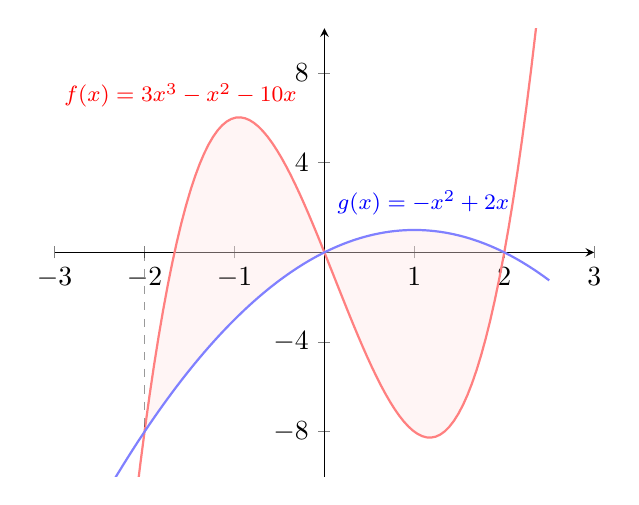
\begin{tikzpicture}

   \begin{axis}[
   		xmin=-3, xmax=3,
   		ymin=-10, ymax=10,
   		xtick distance=1, ytick distance=4,
   		axis x line=center,
          axis y line=center, ]

    \addplot [domain=-2.5:2.5, samples=100, name path=f, thick, color=red!50]
        {3*x^3 - x^2 - 10*x};

    \addplot [domain=-2.5:2.5, samples=100, name path=g, thick, color=blue!50]
        {- x^2 + 2*x};

    \addplot[red!10, opacity=0.4] fill between[of=f and g, soft clip={domain=-2:2}];

    \draw [dashed, opacity=0.4] (axis cs:{-2,0}) -- (axis cs:{-2,-8});

    \node[color=red, font=\footnotesize] at (axis cs: -1.6,7) {$f(x)=3x^3 - x^2 - 10x$};
    \node[color=blue, font=\footnotesize] at (axis cs: 1.1,2.2) {$g(x)=- x^2 + 2x$};

   \end{axis}

  \end{tikzpicture}
  
\begin{enumerate}[i)]

\item
\[f(x) = g(x) \Rightarrow 3x^3 - x^2 - 10x = - x^2 + 2x \]
\[3x^3 - x^2 - 10x + x^2 - 2x = 0\]
\[3x^3 - 12x = 0\]
\[x(3x^2-12) = 0\]
\[x_1 = 0 \]
\[(3x^2-12) = 0 \Rightarrow x_{1, 2} = \pm 2\]
\item
\[I_1 = (-2;0) \; I_2 = (0;2)\]
\[A_1 = \int_{-2}^0 f(x)-g(x) dx = \int_{-2}^0 3*x^3 - x^2 - 10*x - (- x^2 + 2*x) dx \] 
\[=\int_{-2}^0 3x^3 - 12x = [\frac34 x^4 - 6x^2]_{-2}^0 = 0-(\frac 34 \cdot 16 - 24)= 12\]
\[A_2 = \int_0^2 g(x)-f(x) dx = \int_0^2 - x^2 + 2*x - (3x^3 - x^2 - 10x)\]
\[ = \int_0^2  -3x^3 + 12x = [-\frac 34 x^4 + 6x^2]_0^2 = -12+24 = 12\]

\item \[A = |A_1|+|A_2| = 12+12 = 24\]

\end{enumerate}


\end{document}